\documentclass{standalone}

% put this in your preamble
\usepackage{tikz}

\begin{document}

% put this tikzpicture block in your LaTeX document where you want the figure
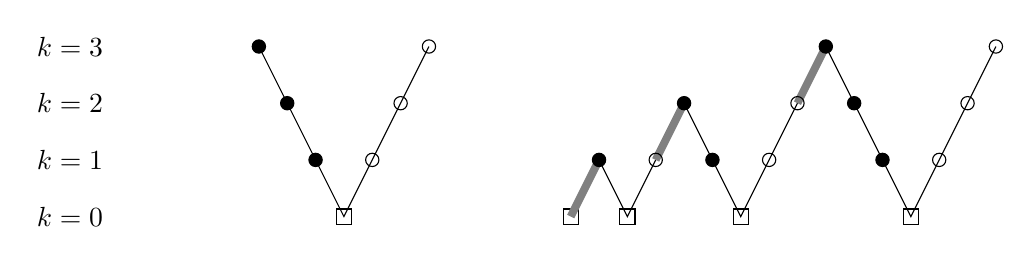
\begin{tikzpicture}[scale=1.2]
  \pgfmathsetmacro\hstep{0.3}
  \pgfmathsetmacro\vstep{0.6}
  \pgfmathsetmacro\ceps{0.08}   % size of square for coarse grid

% grid labels at left
  \node at (-2,3*\vstep) {$k=3$};
  \node at (-2,2*\vstep) {$k=2$};
  \node at (-2,\vstep) {$k=1$};
  \node at (-2,0.0) {$k=0$};

% V-cycle
  \draw[black,thin] (0.0,3*\vstep) -- (\hstep,2*\vstep) --  (2*\hstep,\vstep) -- (3*\hstep,0.0)
                    -- (4*\hstep,\vstep) -- (5*\hstep,2*\vstep) -- (6*\hstep,3*\vstep);
  \filldraw (0.0,3*\vstep) circle (2.0pt);
  \filldraw (\hstep,2*\vstep) circle (2.0pt);
  \filldraw (2*\hstep,\vstep) circle (2.0pt);
  \draw     (3*\hstep-\ceps,-\ceps) rectangle (3*\hstep+\ceps,+\ceps);
  \draw     (4*\hstep,\vstep) circle (2.0pt);
  \draw     (5*\hstep,2*\vstep) circle (2.0pt);
  \draw     (6*\hstep,3*\vstep) circle (2.0pt);

% initial coarse solve
  \pgfmathsetmacro\hoff{11*\hstep}
  \draw[shift={(\hoff,0)}]     (-\ceps,-\ceps) rectangle (+\ceps,+\ceps);
  \draw[line width=1mm,gray,shift={(\hoff,0)}] (0.0,0.0) -- (\hstep,\vstep);

% V-cycle to level 1
  \pgfmathsetmacro\hoff{12*\hstep}
  \draw[shift={(\hoff,0)},black,thin] (0.0,\vstep) -- (\hstep,0.0) -- (2*\hstep,\vstep);
  \draw[line width=1mm,gray,shift={(\hoff,0)}] (2*\hstep,\vstep) -- (3*\hstep,2*\vstep);
  \filldraw[shift={(\hoff,0)}] (0.0,\vstep) circle (2.0pt);
  \draw[shift={(\hoff,0)}]     (\hstep-\ceps,-\ceps) rectangle (\hstep+\ceps,+\ceps);
  \draw[shift={(\hoff,0)}]     (2*\hstep,\vstep) circle (2.0pt);

% V-cycle to level 2
  \pgfmathsetmacro\hoff{15*\hstep}
  \draw[shift={(\hoff,0)},black,thin] (0.0,2*\vstep) --  (\hstep,\vstep) -- (2*\hstep,0.0) -- (3*\hstep,\vstep) -- (4*\hstep,2*\vstep);
  \draw[line width=1mm,gray,shift={(\hoff,0)}] (4*\hstep,2*\vstep) -- (5*\hstep,3*\vstep);
  \filldraw[shift={(\hoff,0)}] (0.0,2*\vstep) circle (2.0pt);
  \filldraw[shift={(\hoff,0)}] (\hstep,\vstep) circle (2.0pt);
  \draw[shift={(\hoff,0)}]     (2*\hstep-\ceps,-\ceps) rectangle (2*\hstep+\ceps,+\ceps);
  \draw[shift={(\hoff,0)}]     (3*\hstep,\vstep) circle (2.0pt);
  \draw[shift={(\hoff,0)}]     (4*\hstep,2*\vstep) circle (2.0pt);

% V-cycle to finest (level 3)
  \pgfmathsetmacro\hoff{20*\hstep}
  \draw[shift={(\hoff,0)},black,thin] (0.0,3*\vstep) -- (\hstep,2*\vstep) --  (2*\hstep,\vstep) -- (3*\hstep,0.0)
                    -- (4*\hstep,\vstep) -- (5*\hstep,2*\vstep) -- (6*\hstep,3*\vstep);
  \filldraw[shift={(\hoff,0)}] (0.0,3*\vstep) circle (2.0pt);
  \filldraw[shift={(\hoff,0)}] (\hstep,2*\vstep) circle (2.0pt);
  \filldraw[shift={(\hoff,0)}] (2*\hstep,\vstep) circle (2.0pt);
  \draw[shift={(\hoff,0)}]     (3*\hstep-\ceps,-\ceps) rectangle (3*\hstep+\ceps,+\ceps);
  \draw[shift={(\hoff,0)}]     (4*\hstep,\vstep) circle (2.0pt);
  \draw[shift={(\hoff,0)}]     (5*\hstep,2*\vstep) circle (2.0pt);
  \draw[shift={(\hoff,0)}]     (6*\hstep,3*\vstep) circle (2.0pt);
\end{tikzpicture}
\end{document}
